\section{Theory of Operations}

\subsection{Introduction}
The \textbf{DynamicFifo} is a highly parameterized FIFO and FIFO controller. It
is configurable as a full self-contained FIFO with internal memory being 
constructed from flip-flops, or a FIFO controller that uses an external SRAM 
for memory.

\begin{figure}[h]
  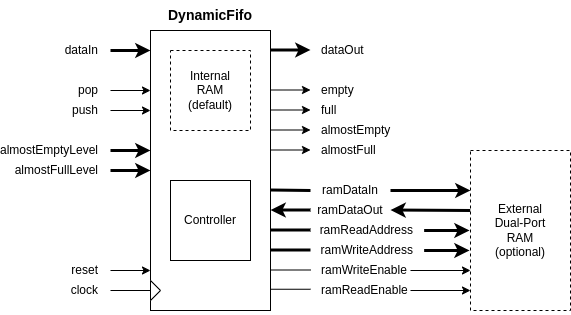
\includegraphics[width=0.80\textwidth]{images/block-diagram.png}
  \caption{Block Diagram}\label{fig:block-diagram}
\end{figure}

It features the following status flags which are described in
Table~\ref{table:ports}.

\begin{itemize}[noitemsep]
  \item{empty}
  \item{full}
  \item{almostEmpty}
  \item{almostFull}
\end{itemize}

When \textit{push} is asserted, the data on the \textit{dataIn} port is enqued
on the next rising edge of \textit{clock}. When \textit{pop} is asserted, the
top of the FIFO is dequed on the next rising edge of \textit{clock} Pop and Push
operations can be simulataneous.

There are two error conditions which produce the following effects:
\begin{itemize}
  \item{When \textit{pop} is asserted and the FIFO is empty (\textit{empty} is
        active), \textit{dataOut} will contain the last valid data held in
        the FIFO.}
  \item{When \textit{push} is asserted and the FIFO is full (\textit{full} is
        active), \textit{dataIn} will be ignored and not enqued.}
\end{itemize}

The \textit{almostEmpty} and \textit{almostFull} flags allow for additional
feedback to the system that is useful for optimizing data flow control. The
levels of these flags can be programmed dynamically through the
\textit{almostEmptyLevel} and \textit{almostFullLevel} ports.

\newpage
\subsection{Interface Timing}

DynamicFifo has a simple, synchronous interface. The timing diagram shown below
in Figure~\ref{fig:timing} represents an instantiation with the following 
parameters.

\begin{lstlisting}[language=Scala]
val myFifo = new DynamicFifo(
  externalRAM = true, 
  dataWidth = 16, 
  fifoDepth = 5) 
\end{lstlisting}

\begin{figure}[h]
  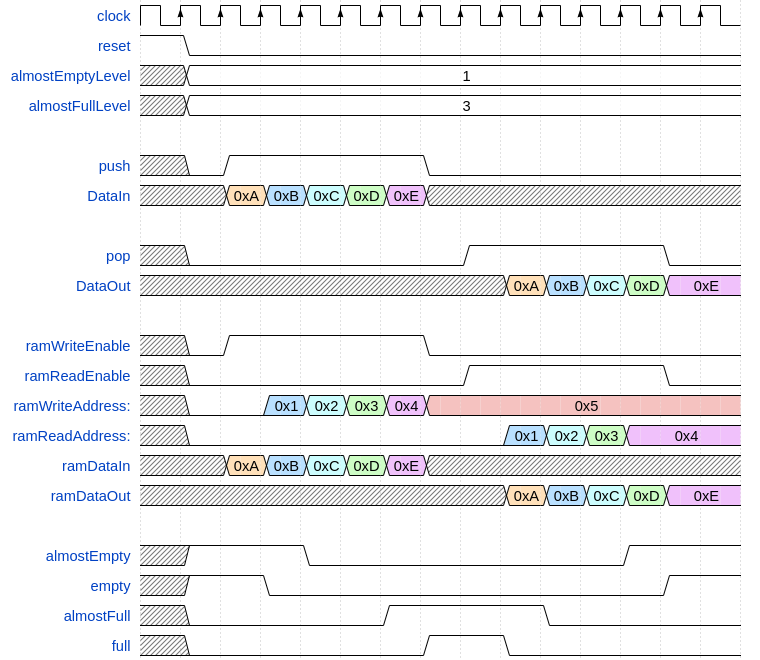
\includegraphics[width=\textwidth]{images/timing.png}
  \caption{Timing Diagram}\label{fig:timing}
\end{figure}

The \textit{almostEmptyLevel} port is driven by external logic to a static value 
of 1 after reset and the \textit{almostFull} port is driven to 3.

Beginning in the third clock cycle, 5 words of data are pushed into the 
FIFO.\ The status flags show the FIFO going from empty to full.

The FIFO is then fully emptied when the \textit{pop} port is help high for
5 clock cycles. The status flags show the FIFO going from full to empty again.